\chapter{机器学习的基本概念与任务}
\label{chap:concepts}
\chaptergoal{学完本章，应能从一张具体数据表中指出样本、输入特征和目标；用自己的话解释模型、训练与预测；区分监督学习与无监督学习，以及分类、回归、聚类和降维任务。阅读本章不需要预先认识任何机器学习算法。}

假设实验室已经记录了不同输入信号下传感器的输出。现在输入一个新的信号，我们希望在测量之前估计传感器将给出什么数值。又假设已经测量了一批花的尺寸，并由专家确定了它们的物种；面对一朵尚未辨认的花，我们希望根据尺寸判断其物种。这两个问题的对象不同，但都希望借助已有记录，对新对象作出判断。

本章从这些具体问题开始。我们先读懂数据，再为其中的对象和操作命名。代码只是把思路交给计算机的表达方式；在知道数据是什么、要解决什么问题之前，不需要急于训练一个模型。

\section{从天文与物理问题到机器学习任务}
\subsection{什么是机器学习}
\textbf{机器学习（machine learning）是利用已有数据，按照明确的学习目标建立或调整计算规则，以完成预测、识别或数据结构分析的一类方法。}这里的“学习”不是计算机理解了对象的全部含义，而是规则的某些部分由数据确定，而非全部由人逐条写出。

例如，人可以先规定“输入信号每增加一个单位，预测输出增加两个单位”。这是一条人工给定的规则。另一种做法是收集输入与输出的配对记录，让计算程序寻找一条较贴近这些记录的直线。后一种方法中，直线的斜率和截距由数据决定，是本书讨论的数据学习过程。选择什么形式的规则、依据什么标准认为它合适，仍需要人作出规定。

一组为某项分析整理在一起的数据记录称为\textbf{数据集（dataset）}。数据集可以是表格、图像集合或一系列测量曲线。本书首先使用表格：一行记录一个分析对象，一列记录对象的一项信息。表格的含义由任务决定，不是所有列都要送入模型。

\subsection{先说清要完成什么工作}
在天文学中，可以根据天体在不同波段的亮度判断它是恒星还是星系。恒星是类似太阳的发光天体，星系则由大量恒星、气体等构成；这里希望预测的是一个类别。在物理实验中，可以根据气流速度、声波频率等条件预测测得的声压级；这里希望预测的是一个数值。还可以只观察一批测量记录，寻找彼此相似的群体，而不预先告诉程序每条记录属于哪一类。

这些不同的要求称为\textbf{任务}。预测类别、预测数值和寻找群体不是同一个任务，所需数据和评价方式也不同。暂时不必记住所有算法名称；首先把问题写成一句能检查的陈述，例如：“输入一朵花的四项尺寸，输出三个已知物种中的一个。”

物理理论和机器学习可以共同服务于研究。理论模型通常依据物理假设写出关系；数据模型依据已有记录确定预测规则。两者都需要检查适用范围。即使一个规则能够预测观测结果，也还需要另外的证据才能把它解释为物理机制。本章先学会建立预测问题，科学解释在第16章展开。

\subsection{把科学问题改写成可以检验的任务}
“研究恒星”是研究方向，还不是一个机器学习任务；“从一段光变曲线判断是否具有某类周期变化”才逐渐接近可以实施的问题。要继续说明曲线在什么时段获得、包含多少个测量点、参考类别怎样确定，以及以后遇到的新对象与现有对象有何关系。\textbf{任务的精确程度，决定了后面每一个技术选择是否有意义。}

以温度传感器为例，我们有两种不同需求。需求甲是根据传感器电压估计参考温度，部署时能测到电压，但不能总是使用昂贵的参考仪器。需求乙是根据已知温度、输入电压和仪器编号预测输出，检查设备是否偏离正常工作状态。两者都涉及相似的测量表，但预测目标不同，能够使用的输入也不同。不能因为表格相同，就沿用同一个任务描述。

\worked{一个可执行的任务说明}
假设实验室已在20件传感器上测量电压和参考温度，每件重复测量10次。现要给\emph{新的传感器}标定。样本表虽然有200行，独立设备只有20件；输入为部署时可得到的电压和环境温度，输出为参考仪器测得的温度。评价应让某些整件设备不参与建模，再检查对这些设备的预测。这是一个人为设定的任务，不是本书的真实仪器实验。

若目的改成给\emph{同一件已经见过的传感器}预测下一次测量，就可能使用该设备过去的记录。前者检查跨设备迁移，后者检查同设备上的重复应用。没有任何一种划分天然适用于两种目标。读者此时无需掌握具体拆分函数，但应能发现“样本到底是什么”和“将来会预测谁”是方法的一部分。

\subsection{预测关系不等于物理关系，二者仍可以协作}
一个模型可以先用物理分析构造有意义的输入，再用数据估计未知系数。例如运动学提示位移可能与时间和时间平方有关，回归程序负责估计相应系数。反过来，数据残差的系统变化也可以提示某个物理假设不充分。机器学习并不要求放弃专业知识，也不保证从未经整理的原始表中自动找到研究对象的本质。

本书区分三个层次。\textbf{预测层次}问新样本结果是否准确；\textbf{描述层次}问现有数据中哪些变量一起变化；\textbf{解释层次}问改变某个物理条件是否会导致结果改变，以及机制是什么。三者可能相互支持，但需要的证据不相同。例如仪器编号帮助识别设备，未必意味着编号本身决定测量值。后续章节中的模型分数首先属于预测层次。

\section{样本、特征、标签与目标变量}
\label{sec:iris-intro}
\subsection{先认识一组花的测量记录}
我们从\textbf{鸢尾花测量数据集（Iris dataset，后文简称鸢尾花数据）}开始。Iris 是这一数据集的英文名称，不是算法。数据中有150条花的测量记录，来自三个物种，每个物种50条；每条记录有四项尺寸测量，单位均为厘米。三个物种以 \textit{Iris setosa}、\textit{Iris versicolor} 和 \textit{Iris virginica} 记录。无需记忆拉丁名称，只需把它们看作三个不同类别。数据规模、字段与类别对应关系见官方数据说明\textsuperscript{[2,26]}。

四项尺寸是萼片长度、萼片宽度、花瓣长度和花瓣宽度。萼片与花瓣是花的两类结构；本例只需要理解它们被分别测量，不要求植物学知识。表\ref{tab:iris-records}摘取了三条实际记录。这里的“记录行号”仅用于找到这条记录，不是花的一项尺寸。

\begin{table}[htbp]\centering\small
\caption{鸢尾花数据中的三条记录。四项尺寸的单位均为厘米；编号为随书数据的零起始位置。}\label{tab:iris-records}
\begin{tabular}{rrrrrl}\toprule
记录行号&萼片长&萼片宽&花瓣长&花瓣宽&已知物种\\\midrule
0&5.1&3.5&1.4&0.2&setosa\\
50&7.0&3.2&4.7&1.4&versicolor\\
100&6.3&3.3&6.0&2.5&virginica\\\bottomrule
\end{tabular}
\end{table}

读第一行时，可以把它说成一句话：“这朵花的萼片长5.1厘米、宽3.5厘米，花瓣长1.4厘米、宽0.2厘米，已知物种为setosa。”表格中的数字和物种不是彼此独立的清单：它们属于同一朵花，必须保持对应。

\subsection{给数据表中的角色命名}
\textbf{样本（sample）}是本次分析中的一条对象记录。在本例中，一朵花的测量记录是一个样本，150行就是150个样本。\textbf{特征（feature）}是用于作出预测的输入信息；这里四项尺寸是四个特征。\textbf{目标变量（target）}是希望模型预测的量；这里希望预测物种，所以物种是目标。对于这种类别目标，本书也称其为\textbf{类别标签（class label）}。

“特征”和“目标”不是一个字段永远不变的属性，而是它在当前任务中的角色。如果问题改为根据其他尺寸预测花瓣长度，花瓣长度就成为目标，不再同时作为该任务的输入。每次建模都应先确定任务，再分开输入与目标。

用 $\mathbf x_i$ 表示第 $i$ 条记录的四个输入，第一行可写为
\[
\mathbf x_1=(5.1,3.5,1.4,0.2),\qquad y_1=\text{setosa}.
\]
这里下标1表示书写中的第一个样本，与表中零起始的程序行号0对应。把所有样本的输入逐行排列，得到\textbf{特征矩阵} $X$；把对应目标依次排列，得到目标序列 $y$。若有 $n$ 个样本、$p$ 个特征，$X$ 有 $n$ 行、$p$ 列，记作 $X\in\mathbb R^{n\times p}$。鸢尾花数据的输入形状就是 $(150,4)$，而不是 $(150,5)$；类别列不包含在输入矩阵中。

\subsection{数字编码不改变字段的含义}
程序可以把三个物种编码为0、1、2。它们只表示类别身份，不表示第三类比第一类“多两单位”，也不意味着类别1位于类别0与类别2之间。预测类别时，应核对数字与名称的对应关系，不能仅根据数字形式就把目标当作连续测量量。

一张专业表还可能有编号、测量时间和质量说明。编号用来识别对象，质量说明用来判断测量是否可靠，它们不一定作为预测输入。一个天体有三次观测时，表中可能出现三行，但只有一个科学对象。第一次读表就应知道“一行代表什么”，更复杂的分组问题留到第4章。

\subsection{一行数据与一个对象：重复测量为什么需要单独登记}
数据中的一行可以代表一件对象，也可以代表对象的一次测量。在天体目录中，\texttt{object\_id}可以识别天体，\texttt{observation\_id}识别一次观测；两者不能互相代替。一个对象被观测多次时，这些行可能共享几乎相同的真实物理性质。把所有行数直接当作独立对象数，会夸大数据提供的新信息。

第一次建立数据表时，可以让每行同时带有“行标识”和“对象标识”。前者用于追踪程序中的预测，后者用于识别相关测量。它们都不必自动进入模型。程序需要这些字段来保证可追踪性，模型则只接收任务允许的输入。\textbf{保存一列与把一列作为特征，是两个不同决定。}

\worked{把表格写成输入与目标}
用一个人工三行例子练习符号：三次测量的输入电压为1、2、3 V，环境温度为20、20、25摄氏度，参考输出为2.1、4.0、6.2 V。若预测参考输出，则
\[
X=\begin{pmatrix}1&20\\2&20\\3&25\end{pmatrix},\qquad
\mathbf y=\begin{pmatrix}2.1\\4.0\\6.2\end{pmatrix}.
\]
矩阵是三行两列，所以$n=3,p=2$。第2行的输入为$(2,20)$，不能与第3行目标6.2拼成一对。数据排序、删除缺失行或合并表格时，必须保持这种配对。机器学习程序通常无法从数值本身判断配对是否已经错位。

此时还没有学习模型。矩阵只是一种组织输入的方式；同一个$X$可以交给不同模型。把矩阵写出来有助于检查数据形状，但不会替代对每列的单位和含义的说明。

\section{模型、训练、预测与泛化}
\subsection{模型是一条可以计算的规则}
\textbf{模型（model）}是从输入产生输出的可计算规则。比如，给定一个长度 $x$，直线规则 $\hat y=ax+b$ 会给出一个预测值。给定一朵花的尺寸，一组条件判断也可以给出一个预测物种。帽子符号 $\hat y$ 表示预测结果；不带帽子的 $y$ 表示数据中用于对照的目标。

\textbf{模型参数（parameter）}是规则内部可由数据确定的量。直线中的斜率 $a$ 和截距 $b$ 就是两个参数。先规定使用直线，再改变这两个数，可得到不同的具体模型。不要把参数与输入混淆：输入是要预测的对象提供的信息，参数则是模型已经学到并保存的规则组成。

\textbf{算法（algorithm）}是完成某项计算的一组步骤。学习算法说明怎样根据数据确定模型，训练后的模型则是可用于新输入的具体规则。比如“用最小二乘计算直线系数”描述算法，求得系数后的一条具体直线描述模型。统一的软件接口不表示所有算法采用同一种学习过程。

\subsection{训练、预测和评价是三种操作}
\textbf{训练（training，也称拟合）}是学习算法根据训练数据确定模型的过程。\textbf{预测（prediction）}是把新输入交给已经确定的模型，计算它的输出。\textbf{评价（evaluation）}是按事先规定的标准比较预测与参考信息，检查模型完成任务的程度。

可以把过程想成“看例题建立做题方法，然后独立做新题，最后核对答案”。这个类比只用于区分数据的用途：模型并不像人一样理解题意，它依照规定的计算程序工作。

\begin{table}[htbp]\centering\small
\caption{以花的物种判断为例，训练与预测使用的信息不同。}
\begin{tabularx}{\linewidth}{p{0.12\linewidth}XX}\toprule
操作&程序使用的信息&产生的结果\\\midrule
训练&一批花的四项尺寸和对应的已知物种&确定一套判断规则\\
预测&待判断花的四项尺寸&给出预测物种\\
评价&保留记录的预测物种及参考物种&统计判断正确或错误的情况\\\bottomrule
\end{tabularx}\end{table}

\textbf{泛化（generalization）}指模型对未参与学习、且属于目标应用范围的新样本完成任务的能力。记住150条已有记录，并不自动意味着能判断第151朵花。为了初步检查这一点，我们可以把部分已知记录保留下来，训练时不使用它们，预测时也不把其物种交给模型；直到评价时才用这些物种核对答案。

图\ref{fig:supervised-intro}把输入、目标和模型的角色分开。图中的“参考目标”进入训练与评价环节，但不作为待预测对象的输入。第3章介绍怎样寻找参数，第4章介绍怎样划分和评价数据。
\begin{figure}[htbp]\centering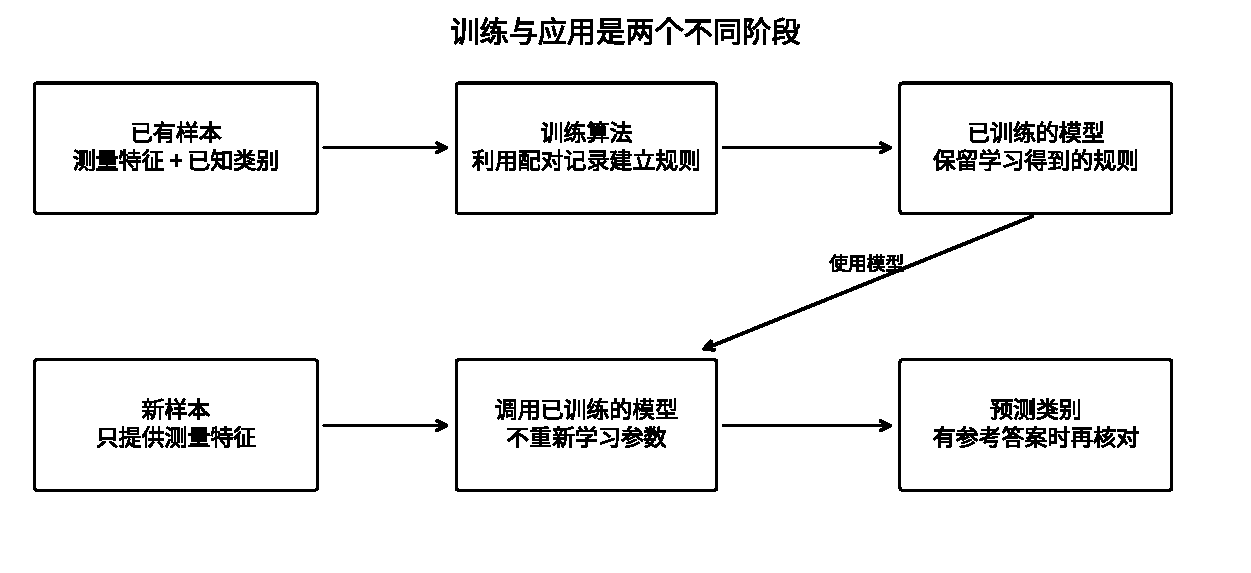
\includegraphics[width=0.92\linewidth]{figures/v2_supervised_flow.pdf}\caption{监督预测的学习与应用过程。标签在训练时提供学习依据，在评价时用于核对，不作为新样本预测的输入。}\label{fig:supervised-intro}\end{figure}

\subsection{学到规则和记住记录的区别}
设训练记录只有输入1、2、3，目标分别为3、5、7。规则甲保存三条记录，遇到完全相同的输入就返回对应目标；规则乙采用$\hat y=2x+1$。两者在已有记录上的预测相同，但对$x=2.5$，规则甲还需要额外规定如何处理，规则乙给出6。\textbf{训练数据上的一致表现，不足以唯一决定新输入上的行为。}

任何模型都包含关于新情况如何延续的假设。直线模型假设关系可以用固定斜率描述；近邻模型假设附近输入往往有相似目标；树模型假设可以通过若干阈值把输入空间分成较简单的区域。这类方法倾向在后面逐章解释。先认识到“数据告诉了什么”和“方法另外假设了什么”，才能理解为什么不存在对所有任务都最好的模型。

对于完全相同的输入却有不同目标的记录，模型也无法逐条区分。例如两条记录都是$x=2$，目标却是4和6，任何只看$x$的确定性规则都只能给出一个数。这可能来自测量噪声，也可能因为输入遗漏了重要条件。增加优化次数不会自动创造缺失的信息。第3章讨论怎样在这些目标之间折中，第16章讨论怎样区分噪声和可改善的模型误差。

\section{监督学习中的分类与回归}
\label{sec:supervised-definition}
\subsection{“监督”来自哪里}
\textbf{监督学习（supervised learning，也称有监督学习）是利用输入与已知目标成对出现的训练记录，学习从输入到目标的预测关系的一类方法。}“监督”指目标提供了学习所依据的信息，不是有人在程序运行时逐次指导，也不要求训练过程的每一步由人干预。

在花的例子中，程序同时获得尺寸与物种。它可以据此确定哪些特征组合有助于区分类别。我们已经知道部分答案，是为了学习以后怎样判断尚不知道答案的对象。训练时有目标与预测时目标未知并不矛盾，正是两个阶段的分工。

第8章的树模型根据类别组成选择划分规则；第6章的概率模型根据预测与目标之间的差异调整参数。它们都是监督学习，但内部学习过程不同。监督与否取决于训练使用的信息，不取决于是否调用某个软件函数，也不取决于是否使用梯度下降。

\subsection{分类：目标是类别}
\textbf{分类（classification）}是从一组已定义的类别中，为输入样本预测类别的任务。鸢尾花例子有三个可能物种，属于多分类。只区分“某物种”与“不是该物种”，就是二分类。类别之间可以有自然顺序，也可以没有；本书首先学习没有大小次序的类别识别。

一条记录的分类结果可能正确，也可能错误。后面的概率分类器还会输出对不同类别的支持程度，但此时先理解最基本的结果：预测物种与参考物种是否相同。

\subsection{回归：目标是数值}
\textbf{回归（regression）}是预测数值目标的任务，例如根据输入信号估计传感器输出。目标有大小和差值的意义，预测2.1与2.2的差别可以用相应单位解释。回归并不特指直线拟合，也不要求目标没有测量噪声。

本书采用\textbf{加州住房价值数据集（California Housing）}作为主要回归案例。每条记录对应一个人口普查街区组，即由若干住户构成的统计区域，而不是一套房屋。输入描述区域收入、住房、人口和位置；目标是该区域住房价值的中位数，数值以十万美元为单位。例如目标2.0表示20万美元。数据来自历史人口普查，用于学习建模，不是当前房价资料。具体字段在第5章逐项介绍\textsuperscript{[10]}。

如果模型给某区域预测2.2而参考目标为2.0，预测偏高0.2，即2万美元。这与把物种代码2预测为0不同：前者有可解释的数值差，后者是类别判断错误。任务类型要依据目标的含义判断，不能只看目标列是否存成数字。

\subsection{目标标签从哪里来，为什么也需要检查}
“已知目标”表示在当前数据中提供了可用于学习的参考，不表示参考一定无误。花的物种可以由人工鉴定给出，实验温度可以由参考仪器测量，天体类别可以由已有目录提供。每种获取方式都有适用条件和可能的误差。只有理解标签来源，才能知道模型实际上在学习什么。

例如，把已有分类程序的结果当作标签，新的模型首先是在学习复现该程序的判定，而不是直接获得了独立的物理真相。它可能具有速度或使用成本上的价值，但验证时应区分“与原程序一致”和“与独立可靠身份一致”。同样，把两种参考测量拼接成目标时，要检查单位、零点和量程是否一致。

\worked{同一测量量，可以导出不同任务}
考虑目标温度$T$。直接预测$T$是回归；把$T<0$定义为“低于冰点”、其余为“未低于冰点”，则变成二分类。二者都可以采用监督学习，但评价不同：回归关心偏差多少度，分类关心是否跨过指定界限。一次从$-0.1$预测成$0.1$摄氏度的误差很小，却可能改变类别；从30预测成32摄氏度误差更大，却未必改变这个二分类结果。

因此，不能脱离任务讨论一个误差是否严重。选择分类有时便于决策，但同时丢掉了数值差别；选择回归保留更多数值信息，却需要另外规定行动阈值。这是问题定义阶段应作出的判断，不是某个算法名称自动决定的。

\section{无监督学习中的聚类与降维}
\label{sec:unsupervised-definition}
\textbf{无监督学习（unsupervised learning）是在训练时不使用与样本配对的目标标签，而根据输入数据及事先规定的准则寻找结构或学习表示的一类方法。}它不是“没有任何规则地让程序随意探索”。分析者仍要决定使用哪些特征、怎样衡量相似、希望获得怎样的输出。

\subsection{同一数据，可以提出不同问题}
现在仍然使用花的四项尺寸，但把已知物种列暂时放在一旁，不交给算法。我们问：“哪些花在尺寸上相似，能否把它们组成几个群体？”根据相似关系形成群体的任务称为\textbf{聚类（clustering）}，所得群体称为\textbf{簇（cluster）}。

监督分类利用已定义的物种学习判断规则；聚类没有利用物种作为训练答案，而是依据输入的相似结构分组。因此，聚类中的“第0组”只是一组样本的编号，不天然对应物种代码0。即便分成三组，也不能直接断定它们就是三个物种。完成聚类后，可以把原有物种拿回来作对照，但这一步与训练时使用标签不同。

\subsection{降维：用较少变量重新表示样本}
每个样本的输入变量数称为其特征\textbf{维数}。四项尺寸给出四维表示。如果其中某些尺寸随花的整体大小一起改变，我们可能希望用少量组合变量概括主要变化。\textbf{降维（dimensionality reduction）}就是把数据变换为较少变量的表示，同时尽可能保留与所选目标有关的信息。

例如把四项尺寸变成两个组合值，便于在平面上画出样本分布。聚类回答“哪些样本应分在一起”，降维回答“怎样用更少的变量表示样本”，两者不能互换。第13章介绍一种具体的降维方法，第14章介绍聚类方法。

\begin{table}[htbp]\centering\small
\caption{学习方式与任务的区别。前者说明训练使用什么信息，后者说明希望输出什么。}
\begin{tabularx}{\linewidth}{p{0.16\linewidth}p{0.24\linewidth}XX}\toprule
学习方式&训练信息&任务例子&输出\\\midrule
监督学习&输入与对应目标&花的物种判断&一个已定义的类别\\
监督学习&输入与对应目标&区域住房价值预测&一个数值\\
无监督学习&不使用目标标签的输入&按花的尺寸寻找群体&群体划分\\
无监督学习&不使用目标标签的输入&压缩尺寸的表示&较少的组合变量\\\bottomrule
\end{tabularx}\end{table}

\subsection{没有标签时，怎样知道分析是否有用}
无监督学习没有提供唯一的参考答案，评价必须更紧密地联系用途。若希望压缩图像，可以检查重构图像丢失了哪些结构；若希望发现观测群体，可以检查相似分组在改变样本或测量误差后是否仍然存在，还可以检查没有参与分组的物理量是否呈现一致关系。

例如把花按尺寸分成两组，可以得到“大花与小花”的描述；分成三组可能更接近物种，也可能仍然混合。仅仅让算法返回更多组，会使每组内部更相似，却不代表科学解释更好。后面的聚类章节会明确区分“数学准则较好”和“符合我们关心的结构”。

已有标签仍然可以用作事后对照。关键是不要反复用这些标签调节无监督参数，然后仍声称标签从未影响分析。如果已经这样选择参数，整个流程就利用了标签信息。学习方式应按完整的信息流描述，而不是只按最后一个函数的名称分类。

\section{半监督、自监督与强化学习概览}
\textbf{半监督学习（semi-supervised learning）}同时利用少量有标签记录和较多没有标签的记录。例如，只辨认了一部分花的物种，但测量了更多花的尺寸；方法可以同时利用两部分数据。无标签记录怎样帮助学习，依赖额外假设，并非加入它们必然改善结果。

\textbf{自监督学习（self-supervised learning）}从数据自身构造学习目标。例如，遮住一幅图像的一部分，利用保留部分预测被遮住的内容。目标由已有数据产生，不需要人为逐条提供类别；但训练仍然有明确的预测任务和比较标准。

\textbf{强化学习（reinforcement learning）}研究行动者通过与环境交互，学习怎样行动以获得较大的长期累计奖励。行动者称为智能体，行动结果影响后续环境状态。例如一个简化的移动控制任务中，程序选择移动方向，环境返回位置和奖励；问题不仅是判断固定记录，还包括行动怎样影响以后能够获得的信息和结果。

这三类方法仅作概览，不是本课程的算法主线。它们可以在同一应用中组合，名称并不总是相互排斥。判断一段学习过程时，先看实际提供了什么信息、优化什么目标，再使用术语描述。

\section{一次完整机器学习任务的基本流程}
\subsection{先把过程讲清，再看软件}
对花的分类，一个完整入门实验可以按以下顺序进行：先明确输入为四项尺寸、目标为物种；检查记录与标签的对应；把一部分样本留作评价；用其余样本建立判断规则；只根据保留样本的尺寸预测物种；最后核对预测与参考物种，记录正确和错误的例子。代码应当能逐步对应这些操作。

本书使用\textbf{scikit-learn}，这是一个提供机器学习算法及数据处理、评价工具的Python软件包。在Python中导入它时使用模块名 \texttt{sklearn}；两种写法指向同一个工具。它与“监督学习”等方法概念不同，也与“鸢尾花数据”等具体资料不同。\texttt{load\_iris()} 是取得鸢尾花记录的函数，名称中的 \texttt{load} 表示读取；调用它不等于已经训练模型\textsuperscript{[26,30]}。

\begin{lstlisting}[caption={只读取已介绍的鸢尾花数据，不进行训练}]
from sklearn.datasets import load_iris
flowers = load_iris(as_frame=True)
X = flowers.data
y = flowers.target
print(X.shape, y.shape)
\end{lstlisting}

\noindent 上面代码中的输入对象在第2章将完整读入为表格。这里先用最少的读取语句区分“取得数据”和“根据数据学习”：创建变量 \texttt{flowers} 只是保存返回结果；\texttt{flowers.data} 是尺寸表。目标保存在 \texttt{flowers.target} 中，类别名称保存在 \texttt{flowers.target\_names} 中。表格操作及输出解释都在下一章展开，暂时不需要记忆所有接口。

\fig{ch01_workflow.pdf}{机器学习任务的完整流程概览。图中的模型选择是比较候选规则，最终评价是在规则确定后检查保留数据；具体操作将在第4章解释。}

\subsection{用一句完整的话描述你的任务}
一个可以开始实施的任务至少说清四件事：一条样本代表什么；预测时能获得哪些输入；希望输出什么；怎样检查输出是否有用。以花的例子为模板：“每条样本是一朵花；输入为四项尺寸；输出为物种；用训练时未使用的花检查物种判断是否正确。”

接触科学数据时，继续补充输入和目标的来源。例如，根据多波段亮度判断天体类别时，不同波段指不同波长范围内的亮度测量；参考类别可以来自更详细的光谱分析。此时就要区分用于预测的信息与用于提供参考答案的信息，而不是把表中每一列都投入模型。

\subsection{第一次完成一个小任务，不必立即理解所有算法}
下面的实验只使用已经认识的鸢尾花尺寸，先比较两个能读懂的判断规则。规则一对每朵花都报告训练部分中更常见的二分类结果；规则二规定“花瓣长度小于2.5厘米时报告setosa，否则报告非setosa”。后一阈值在这里是\emph{预先规定的教学规则}，不是通过本次验证数据寻找的最优值，也不作为正式的物种鉴定结论。

随书脚本先按固定随机种子保留30朵花作最终测试，不读取其结果；120朵开发样本中用90朵作训练、30朵作本次验证。训练部分确定多数类基线。实际运行中，验证30条里基线判断对20条，预先规定的长度规则判断对30条。这个结果说明该尺寸在这一小任务中有区分作用，但没有证明阈值2.5对所有新地区或新测量都有效。

\begin{lstlisting}[caption={把已有规则应用到新的输入，类别信息只用于最后核对}]
petal_length = X_val["petal length (cm)"].to_numpy()
predicted = petal_length < 2.5
reference = (y_val.to_numpy() == 0)
number_correct = (predicted == reference).sum()
print(number_correct, len(reference))
\end{lstlisting}
这段代码中的\texttt{X\_val}和\texttt{y\_val}来自随书完整实验的固定划分。比较发生在预测之后：条件判断只读取花瓣长度，参考物种没有进入判断条件。第4章解释划分方法，第8章把人工规定阈值改成由训练数据选择阈值。这样，已有经验规则、简单基线与学习算法之间的联系就清楚了。

\subsection{检查本章是否真正学会}
读完本章，应该能把任一案例分成三层：现实对象是什么；为完成任务把它表示成哪些数字；程序根据这些数字做什么。没有读懂第一层时，不应急于讨论第三层的算法参数。能够在纸上画出训练与预测的信息流，比提前记住十个模型缩写更重要。

\chapterpractice{先读表\ref{tab:iris-records}，逐项说出样本、输入与目标。再用同一数据描述分类和聚类两个任务，明确哪一步使用类别信息。最后任选一个熟悉的实验或天文问题，写出样本、输入、预期输出及一个检查结果的方法；这一任务只要求定义问题，不要求提前实现算法。}
\chapterexercise
\begin{enumerate}
\item 一张表有150行、4列尺寸和1列物种。用于物种分类的特征矩阵有几行几列？为什么不把物种列同时作为输入？
\item 训练时已经知道花的物种，为什么仍然需要学习分类规则？训练、预测、评价各使用什么信息？
\item 把三个物种编码为0、1、2，是否就变成了回归问题？请说明目标含义与存储形式的区别。
\item 同一批尺寸记录，怎样分别用于分类和聚类？聚类组号为什么不能直接当作物种编号？
\item 在实验记录中，一行是一件材料还是一次测量，为什么需要先说明？写出一个完整的任务定义。
\end{enumerate}

\section*{深化练习与方法检验}
本组题强调解释、计算与验证；D编号在本章内独立计数。计算题应写出所用定义和中间步骤，实验题保留实际输出，包括不支持预期的结果。
\begin{enumerate}[label=D\arabic*.]
\item 某表记录同一传感器在不同输入电压下的读数。任务甲根据输入电压估计输出电压，任务乙根据输出曲线判断传感器是否故障。两者的样本单位、输入和目标是否必然相同？各写一份没有信息泄漏的任务定义。
\item 两个对象的全部输入完全相同，但参考类别不同。一个确定性的分类模型能否同时把两条记录都分对？这说明提高算法复杂度能够解决什么、不能解决什么？
\item 算法先把图像的一部分遮住，学习预测被遮住的像素，再利用少量物种标签进行分类。分别说明两个阶段的学习目标、目标来源，以及两个阶段是否都可以有数值损失。
\item 把鸢尾花物种标签随机打乱后，仍能得到一张格式正确的数据表。此时数据形状检查与科学含义检查分别能发现什么？设计一个不需要复杂算法的核对步骤。
\end{enumerate}
